
\subsection{Description des travaux par t�che / Description by task}
\begin{xcomment}  
Pour chaque tâche, d\'ecrire : 
les objectifs et \'eventuels indicateurs de succ\`es,
les personnes impliqu\'ees,
le programme d\'etaill\'e des travaux,
les livrables,
les contributions des personnes (le qui fait quoi ),
la description des m\'ethodes et des choix techniques et de la mani\`ere dont les solutions seront apport\'ees,
les risques et les solutions de repli envisag\'ees.
\end{xcomment}






\subsubsection{WP1 Kinesics}


\begin{center}
\begin{tabular}{|p{3cm}|p{8cm}|}\hline
WP1 &  Kinesic component \\\hline
Responsable &  LIF  \\\hline
Participants &  Inria, Telecom ParisTech\\\hline
Duration  &  42 months  \\\hline
Objectives &  Develop new generic controlers of a single character alone based on precise spatio-temporal indications of his actions and mood. \\\hline
% Content &  \\\hline
Task 11 & Full body animation  (T0 $\rightarrow$ T0+36) \\\hline
Task12 &  Face and gesture animation (T0+12 $\rightarrow$ T0+36) \\\hline
Task13 &  Learning from few samples (T0+18 $\rightarrow$ T0+42) \\\hline
\end{tabular}
\end{center}



The goal of this WP is to develop new generic models able to produce animation of a single character. It includes designing animation models of a character realizing an action (walking, sitting etc) given a context that consists in a particular mood and in character profile (age, gender) as well as designing models for taking into account the interaction of the character with others (gaze, harm gesture). Moreover we will explore transfer learning strategies for learning these models from few training samples only to ease addition of new getures, actions and moods. 

The workpackage is divided into three subtasks: {\it animation of the full body of a character alone}, {\it animation of the face of a character engaged in dialogue}, and {\it strategies for learning models from few training data}.

 
% \paragraph{Task11} Full body animation


% Choosing representations for full body motion ; representation learning ; transfer learning ; parameterisation of kinesic components. This can include neuro-muscular variables ; also the choice of kinematic trees rooted at the head ; also the grouping of kinematic variables into synergies ; etc. 
% 
% One classical distinction is between world-frame positions and joint angle variables In our case, we are making a strong statement that we will  study kinesic variables for all joints relative to the rigid body frame associated with the actor. This could be the ground floor position of the actor plus a rigid body position associated with the actor?s head.  Thus proxemic variables could be footsteps and head movements ; kinesic variables could be all other joint angles or joint positions in world coordinates.


\paragraph{Task 1.1. Generic full body animation model}


% A first scientific lock lies in the design of generic body controllers able to synthesize the animation of the full body of a character for many settings (combination of action, emotion and actor's profile). 
% It is an elegant way for producing smooth animation of complex motions which usually requires artifical smoothing and postprocessing. It is also a relevant modeling framework for learning from limited datasets. 
% Indeed gathering a dataset including enough training samples for every combination of (action, emotion, actor profile) is unlikely. 
% Defining generic models should allow to maximize the exploitation of the training data for learning, which is a key issue here. 

We will first focus on the design of generic body controllers able to synthesize the animation of the full body of a character (through the sequence of mocap representation) for a given procedural animation scenario as output by WP2, i.e. a sequence of actions realized with a particular mood context and for a specific character profile (morphology, expressivity level). 
% We will first consider that there is one model per action and that the animation produced by such a model should take into account, as inputs, the mood context as well as the character profile context. 
% We will consider modeling frameworks that allow separating the mood components from the profile components so as to enable extrapolating moods to other profiles, and profiles to other moods. 
% To start we will consider that there is one model per action and that the animation produced by such a model should take into account, as inputs, the mood context as well as the character profile context, later on we will investigate one model for all settings (action, mood, charecter profile). 
We will investigate modeling frameworks that allow taking into account the contextual variables (e.g. mood components and actor's profile components) as few inputs which influence the animation. 
Designing models whose output (a synthesized animation) continuously varies with these contextual inputs naturally yield easy generalizing to unseen settings in the training set (e.g. particular combination of action, mood and actor's morphology). We plan to investigate the following lines of research:
% This will enable learning from a limited combination of (mood, profile) settings while allowing extrapolating to any other combination (mood, profile). 
% Whatever the models under investigation we will pay attention to focus on strategies that enable synthesizing smooth transition between successive actions, moods, or gestures. 


% Such generic models would allow learning the animation model for a particular action may be learned from all samples of this action whatever the mood ant the actor's morphology, and from all samples of any action performed with this particular mood.

% We will first explore extending prevous worls on contextual markovian models \cite{Radenen2014, Ding2013, Ding2014} which are a variant of Hidden Markov Models (HMMs) that are parameterized by contextual information (e.g. means of gaussian distributions of the HMM'states are made a function of contextual variables). This will require extending these models to deal with the full body.
% We will first explore extensions of previous promising works (e.g. Radenen 2014). Then we will explore and propose new ways for parameterizing the animation model with few variables related to the emotional state of an actor and more generally to an actor's profile. 

 
% \begin{itemize}  
%   \item 
  Firstly we will explore how to extend {\it contextual markovian models} whose parameters (means of Gaussian distribution, transition probabilities...), are parameterized by (i.e. defined as a function of)  of contextual variables (mood and profile information). One Contextual HMM may be viewed as a continuum of HMMs, one model for every possible value of contextual variables. Recent work has demonstrated such models for the case of locomotion believable controllers, gesture controllers \cite{DBLP:journals/tog/LevineKTK10} and face controllers \cite{Radenen2014, Ding2013, Ding2014}. We will aim to generalize these works to more general action controllers, including such actions as: sitting, standing, walking, grasping, taking and putting objects, in a variety of expressions and moods. These models will serve as a baseline for evaluating new modeling approaches.



%   \item 
  Second, we will investigate the use of {\it (deep) neural networks} and of dynamic versions of these (i.e. recurrent neural nets) which have demonstrated strong abilities to model, to classify and to synthesize complex signals such as speech or handwriting \cite{DBLP:journals/taslp/Abdel-HamidMJDPY14, DBLP:journals/corr/abs-1303-5778, DBLP:conf/interspeech/Abdel-HamidDYJ13, DBLP:journals/spm/LingKZSSQMD15, DBLP:conf/nips/GravesS08, DBLP:journals/corr/Graves13}. 
  These models are related to what is called {\it representation learning} which emerged in the last few years as a key topic in the machine learning community \footnote{See the recently born ICLR conference on Learning Representations at http://www.iclr.cc/} \cite{DBLP:journals/corr/ContardoDAG13}. 
  One main difficulty will be to integrate the use of contextual information as input in order to modify the behaviour of the models. We plan to extend the principle of contextual markovian models to neural nets by investigating ideas like designing bilinear layers in the neural net where weights could be defined as a function of the contextual input, inspired by works like \cite{DBLP:conf/mm/ZhongLL11, DBLP:journals/pami/HutchinsonDY13}.
%   \item 

  At last we will investigate {\it low dimensional state space models} such as neuro muscular based models following ideas like \cite{DBLP:conf/icfhr/FischerPOS14} which aims at recovering from a handwritten signal the sequence of neuromuscular commands that generated the handwriting signal. The underlying idea here is to exploit such models in order to work in a new representation space, the space of neuromuscular commands that generate motion, rather than on the observed motion itself. 
  Although such models have not been used to model complex gestures up to now it is expected that they could be robust enough to provide good estimation of the command sequence. The main advantage of such a change of representation space is an expected reduction of the dimension of this space (as in \cite{DBLP:journals/pami/WangFH08}), enabling easier learning from few samples and transfer learning (as will be investigated in \textbf{task 1.3}).
%   This would be linked to (Gaussian process reference).
% 
% \end{itemize}


\paragraph{Task 1.2. Combining models for face animation } 

The second task focuses on learning models of gesture and facial expressions in dialogue situations. It is dedicated to the combination of animation models, whch is a diifuckt and open question, with a focus on the animation of the face. We will start from available face animation models in the consortium: a mocap based animation \cite{Ding2013}, a video-based animation \cite{TheseINRIA}, and a procedural animation \cite{Greta} (integrated in the GRETA system). 

All of these models types have pros and cons. While statically-driven models are more prone to produce natural looking animation, cognitive
models capture more precisely the semantic emotional behaviors to communicate. These latter ones are often event-driven; that is they compute a behavior only when a given communicative function is specified. Statically driven models produce animation continuously that captures the communicative colour of the message to convey but they have difficulty to compute behaviors which have specific meaning. As a result, virtual agents driven by cognitive-like system are able to convey more precise displays while those driven by statistical models look more natural and lively \cite{DBLP:conf/iva/LeeM12}.

We will explore ways to combine few such animation models which remains an open question today, be it for animating the face ot the full body \cite{...}. We will explore strategies and implement these within the Greta framework where communicative intentions and emotions are represented with the FLM language while multimodal behaviors with BML \cite{DBLP:conf/iva/VilhjalmssonCCCKKMMMPRTWW07}. The merge of multiple animation models may be performed as a weighted blend of the animations produced where the weights might be context dependent and tuned either manually or automatically, alike in \cite{DBLP:journals/tvcg/ShoulsonMKB14}. Alternatively the animation models may be merged earlier, when deciding which kind of motion to launch, or may have asymetric role. For instance, the procedural animation model (or semantically-driven?) might act as the main animation model and use when neccessary animatyions produced by the other models.




% 
% 
% This subtask focuses on learning models of gesture and facial expressions in dialogue situations. Based on previous work on  visual prosody, we would like to learn joint models of gesture and  speech prosody. Ideally, this should be done without MOCAP data, using only audio and video processing, possibly enhanced with depth (kinect). To be continued (Rémi)...

\paragraph{Task 1.3. Learning from few samples}

We will mainly investigate two approches for extending approaches developped in task T1.1 to enable learning from few samples. The first strategy consists in extending the idea of context variables that models of task T1.1 rely on in order to design a global model for all actions.
In the case of markovian model for instance this means that instead of definig one model per action one could define a unique global markovian model where every state would stand for a particular position of the body and performing an action would correspond to following a path (i.e. a state sequence) in this big model. 
Making transition probablities dependent on the action to perform such a big model would be instaiated as an action model by considering a bundle of paths only in this model.  Doing so one could expect that all the training data (whatever the action it corresponds to) could be exploited to learn all the states of this big markovian model, hence implementing some kind of transfer learning between actions. 
A new action would correspond then in a bundle of paths in this model and could be learnt from few samples only. Preliminary works that we did let us expect that such a strategy would work with statistical markovian models \cite{DBLP:conf/icassp/DingRAP13, RadenenThesis}. In this case the above idea could be implementing by introducing new contextual variables, which might be at the simplest on-hot indicators of the action to perform (a vector with zeros everywhere but at the position of the action number). We will first investigate this strategy for contextual markovian models then we will extend this approach to recurrent neural networks.
A related approach will concern the use of using continuous state space models with a low dimensional state space (e.g. corresponding to the degree of freedom of body poses or to the neuro muscular commands) which should permit characterizing a particular motion or gesture as its dynamic in this latent space whose limited dimension would enable learning from few samples.

\paragraph{Deliverables}\\

 bla bla bla



\begin{tabular}{|p{3cm}|p{10cm}|p{1.5cm}|}\hline
Deliverables & Name and content  & Date  \\\hline
L1.1  & Report on the state of the art for statistical models for animation synthesis & \\\hline
L1.2  & First version of the models : Prototype (software) and its documentation (Report on the models deveopped) & T0 + 18 \\\hline
L1.3  & Second version of the models : Prototype (software) and its documentation (Report on the models deveopped)  & T0 + 36 \\\hline
\end{tabular}

\paragraph{Partners' roles}

bla bla

\paragraph{Risks}

The risks are limited. There will not be any problem with availability of datasets. All along the project we will rely as much as possible on existing datasets. For instance Mocap data of considered actions have already been recorded by C. Pelachaud within the project Feder Anipev (http://www.anipev.com/). 
The corpus EMILYA (EMotional body expressIon in daiLY Actions databaseBodily Emotional Actions Behavior) (Fourati, 2014) is constituted of 7 actions performed by 11 actors with 8 emotions. The actions encompass everyday actions such as walking, carrying an object, and sitting. 
The emotions cover the positive and negative spectrum.



\endinput

\subsubsection{WP2 Proxemics}


\begin{center}
\begin{tabular}{|l|l|}\hline
WP2 &  Proxemic component \\\hline
Responsable &  LTCI  \\\hline
Participants &  Inria, ECM\\\hline
Duration  &   42 months \\\hline
Objectives &  Design and development of low-dimensional, multi-character  animation \\\hline
Content &  \\\hline
Task 21 & Communicative behaviours   ($T_0 \rightarrow  T_0+24$)\\\hline
Task22 &  Steering behaviours  ($T_0+12 \rightarrow  T_0+36$) \\\hline
Task23 &  Combination of statistical and procedural models    ($T_0 +24 \rightarrow  T_0+36$) \\\hline
\end{tabular}
\end{center}

In this workpackage we are interested in modeling behaviors of group of agents while conversing and while moving around. We will pay particular attention at the social interaction of the agents during these activities. We will also develop an animation model that incorporates two models: statistical model as developed in WP1 and procedural model developed within the Greta platform.


\paragraph{Task 2.1: Group behaviors during multi-way conversation}


In this task we will model multi-party conversation behaviors. We will focus on turn-taking management. While indication of what the agents would say to whom and when will be provided by a script (Task 3.1 and Task 4.X), the turn-taking model will instantiate which behaviors the agents will display. Gaze, body orientation, position in space are important cues for indicating who has the turn, who wants to keep it, to give it to someone, who is listening, etc.  We will extend an existing turn-taking model \cite{ RavenetCOP14} that is based on Sack's model \cite{SAC74}, that embeds F-Formation \cite{Kendon90}  and that takes into account social attitude of the agents toward each other. This model is implemented as a state machine where the states are defined by the turn-taking and correspond to conversational roles. Transition between states is triggered when an agent changes conversational role. Attitudes vary the behavior of the agents such as their propensity to gaze at others. We will extend this model to simulate different configurations of speech overlap such as terminal overlaps, conditional access to the turn, and choral \cite{Schegloff2000} as well as long silences when nobody takes the turn. We will add further states to encompass more conversational functions (eg greeting, word search). We will also model that transitions from one state to another one can bring the agents of a group to be in the same state (parallel configuration as when greeting each other or laughing together).


\paragraph{Task 2.2 : Group behaviors during stage movements}

This task will model agent behaviors when moving around in the environment,  included such  advanced  steering behaviors as follow, flee, separate, join, merge, enter stage, exit stage, etc. The animation of the virtual agent doing some tasks will be given by WP1. It will not focus on path planning as this information will be provided by a script (Task 3.1 and Task 4.X). Rather it will model how agents perform displacement in social settings. Gaze direction, body orientation and spatial distance to other agents will be computing for different {\em steering behaviors}. These features will be modeled through different synchronization mechanisms: moving in synch, moving ahead, following, etc. They evolve dynamically in function of each other's  positions and orientations in space. The basic animation of the agent, ie without any influence from surrounding agent, is given by WP1. To simulate the dynamic evolution of agent behaviors,  we will make use of Neural Network simulation \cite{Prepin2013} where we can render how behaviors of one actor can act on behaviors of other actors (eg walking powerfully toward an actor with an angry expression will result in moving backward of another actor with a less dominant attitude. Mutual coupling of behaviors will be modeled as emerging from such action-reactive behavior simulation \cite{Prepin2013} ensuring not only the synchronization between actor behaviors but also their mutual influence. 


\paragraph{Task 2.3:  Combination of statistical and procedural models.}

In this task we will develop an animation model that will merge animations coming from statistical model developed in WP1 and procedural model developed in WP2 (Task 2.1 and Task 2.2). This blend is required for the interaction settings where behaviors of the agents are driven by both animation models.  The procedural model relies on forward and inverse kinematic models \cite{huang:2012:EET}. It controls the arms position, gaze direction and body orientation. The statistical model (from WP1) controls the whole body.  Our animation blender model will work at the modalities level and will also incorporate movement propagation; that is how motion of one body part affects other body parts. At first, the animation blender model will merge whole body motion computed by the statistical model as specific body motion computed by the procedural model. More precisely, arms position, gaze direction and body orientation outputted by the procedural model will be viewed as constraints to be reached. These motions will be added onto the animation computed by statistical model; the position of the arms, head and torso computed by the procedural model will overwrite those computed by the statistical model. In a second step, the animation blender model will incorporate propagation of movements. To compute movement propagation we will develop a statistical model that learns which motion is due to action and which motion is due to movement propagation.

\vspace{5mm}

\begin{tabular}{|l|p{10cm}|l|}\hline
Deliverables & Name and content  & Date  \\\hline
L2.1  & Report on the state of the art of proxemics models in computer animation&   $T_0+12$  \\\hline
L2.2  &  First version of the models : Prototype (software) and its documentation (Report on the models developed) & $T_0+24$ \\\hline
L2.3  &  Second version of the models : Prototype (software) and its documentation (Report on the models developed) &  $T_0+36$ \\\hline
\end{tabular}

\paragraph{Partner's roles} This work package  will be coordinated by LITC. Inria  will contribute to tasks 2.2 and 2.3. LIF will contribute to task 3.3.
 
\endinput

\subsubsection{WP3 Authoring}


\begin{center}
\begin{tabular}{|l|l|}\hline
WP3 &  Authoring \\\hline
Responsable &  Inria  \\\hline
Participants &  Paris 8, LIF, Telecom ParisTech\\\hline
Duration  &   36 months \\\hline
Objectives &  Authoring and execution of virtual actor performances  \\\hline
Content &  \\\hline
Task 31 & Specification of the dramatic score language  ($T_0 \rightarrow  T_0+12$)  \\\hline
Task12 &  Authoring tools  ($T_0+12 \rightarrow  T_0+36$)  \\\hline
Task13 &  Real-time animation   ($T_0+12 \rightarrow  T_0+36$)  \\\hline
\end{tabular}
\end{center}


\paragraph{Task 3.1 : Specification of a dramatic score language}

Previous work in autonomous agents has focused on defining non-verbal communication languages at the functional level (what is being communicated) and the behavioral level (how it is communicated using body language). While a consensus has slowly been reached on the behavioral level with the BML language \cite{Kopp2006}, a general framework for describing non-verbal communication at the functional level remains elusive. In DADA, we will take a very different route by giving specifications only for dramaturgic actions, i.e. actions whose purpose is to be played on a stage and communicated to an audience. This will include a choice of verbs (actions, speech acts, movements) and adverbs (moods, attitudes, dramatic effects)  for directing actors ; and a choice of cues acting as synchronization points between actors.

The research problems to be solved in this task include the definition of parallel and sequential behaviors for single, isolated actors; the definition of parallel and sequential behaviors for groups of actors; an intuitive and general  syntax for control the synchronization between them; the choice of non redundant action primitives; and the choice of meaning parameters to be exposed to the director (as opposed to resolved internally by the animation engine). In agreement with the organization of tasks in WP1 and WP2, the specification will clearly separate proxemic and kinesic elements of actor behaviors. Furthermore,  our goal will be to cover both the movements of actors on the stage, and their communicative behaviors during dialogue. 

As a result of this task, we will be proposing an extended notation for theatre performances, akin to a musical score \cite{gagnere2012,ronfard2012,gagnere2015}. For lack of another word, we
will refer to this future notation scheme as  the {\em  dramatic score}. To define the syntax and semantic of the dramatic score, we will draw  on  previous work on the dramaturgical score \cite{Elam2002}, which takes a semiotics approach, and on established stage management practices in the theatre \cite{Maccoy2004}. The proposed specification will be given in the form of a pseudo-natural language that makes sense to the director, and can at the same time be compiled into a machine representation. Internally, the representation will likely be based on Petri nets, which provides an intuitive and general representation of multi-modal, parallel processes with complex synchronization cues ; and at the same time can easily be resolved into hierarchical finite state machines, which can be executed efficiently in a game engine.

The specification  will borrow important terms from the language of theatre \cite{Maccoy2004}:  blockings, cues and prompts,  which we explain briefly now. In theatre, blocking is the precise movement and staging of actors on a stage in order to facilitate the performance of a play, ballet, film or opera. A theatrical cue is the trigger for an action to be carried out at a specific time. A cue sheet is a form usually generated by the stage manager or design department head that indicates information about the cue including execution, timing, sequence, intensity (for lights), and volume (for sound). The stage manager keeps a master list of all the cues in the show and keeps track of them in the prompt book. The Prompt Book is the master copy of the script or score, containing all the actor moves and technical cues,  and is used by the   stage manager to run rehearsals and later, control the performance. Such traditional notions will need to be thoroughly extended to take into account the 
entirely novel situation of computer-controlled virtual actors.

The specification will be delivered in two increments. The first increment will focus on directing individual actors and synchronizing their actions. The second increment will focus on directing groups of actors and synchronizing their actions  within the group, and  across different  groups.

\paragraph{Task3.2 : Authoring tools}

For the DADA platform to be accepted by theatre directors, it is important that we offer authoring tools that make sense to them. 
Although we are targeting  Petri nets as an internal representation, our goal in task 32 will be to hide this internal representation 
from users. Instead, we we will offer three modes of interaction: didascalia, storyboard sketches, and timelines. Didascalia will
be offered as blocks of text with a controled vocabulary and a choice of parameters allowing the director to define cues, actions and their parameters 
in plain text.  Storyboard sketches will be used to represent the actors positions, orientations and trajectories using a combination of floor-plan views 
and audience views. Timelines will be used to set the starting and ending points of performing events by direct manipulation. There will likely be
one timeline per actor per animation component (proxemic behaviors, kinesic actions, kinesic moods, speech acts, etc.).

As a result, the authoring tools will include multimodal interaction with the director: sketching tools for designing actor trajectories and meeting points; 
writing tools for adding didascalia to dialogues; timeline-driven interaction for defining cue points, actions and timing. 

%User interface  for directing actors by sketching stage floor plans and composing the performing score ; 

% Compilation of the language into a finite state machine and/or Petri net ; allowing real-time execution of the dramatic score.


\paragraph{Task 3.3 : Real-time execution of the dramatic score} 

While task 31 focuses on defining the vocabulary and syntax of the dramatic score, and task 32 focuses on implementing 
a score-writing application, the role of task 33 will be to implement a realizer/synthesizer for executing the dramatic score.
This should include real-time combination of proxemic (procedural) and kinesic components of motion ; non-deterministic motion generation ; synchronization to cues ; real-time skinning and advanced 3D animation ; integration of physically-based secondary animation (skin, hair, clothes, etc.).  This includes integration of the GRETA BML realizer with IMAGINE animation ; and real-time integration of the statistical models of motion with the procedural animation components.

Another challenge to be overcome is in combining full body animation and interaction animation at runtime. We believe it will be an important asset for the DADA platform that each performance is unique, and can be controled in real time by cues given by the director.  We will pay particular attention to design models capable of generating real animations. Indeed synthezing from statistical models usually resumes to finding the most likely animation sequence in a given situation, which may yield to too similar and unrealistic animations.  Actually one would be pretty much interested in synthezing animations that are both likely given the learnt statistical models but also exhibiting the variability one can observe in human motion and gestures. Introducing such a stochastic component in the synthesis while maintaining a high quality animation level is not  straightforward and is an open question that we will have to solve.

Special care will be needed for combining the proxemic and kinesic components of animation at runtime along the lines of Mitake et al. \cite{Mitake09}, 
where the degrees of freedom of a virtual character are separated into six parameters for rigid body simulations,  and four parameters for encoding multi-dimensional keyframe animations. Similarly, we would like to hide the complexity of high-dimensional  character animation (with 40-60 degrees of freedom) behind a small number of control parameters. We will extend rigid body simulations  to include proxemic interaction forces in WP2. And we will replace keyframe animations with statistical models learned from data in WP1. 

Another research issue that will be investigated in this task  is the possibility  of  controlling the proxemic components of character animation using the rigid motion of the head, rather than the full body.  Sreenivasa et al. \cite{Sreenivasa09} have proposed inverse kinematics methods for computing  the body motion of a humanoid robot, including footsteps and walking patterns of motion, given its head motion. In the context of DADA, the head motion of the virtual actors could similarly be put under the direct control of the director because it plays such an important expressive and dramatic function. The full body motion could then be computed with the constraints that the actor's head motion matches the director's directions, and the prescribed actions (walking, sitting, standing, etc.) and attitudes (sadly, swiftly, merrily, etc.).


\vspace{1cm}

\begin{tabular}{|l|p{10cm}|l|}\hline
Deliverables & Name and content  & Date  \\\hline
L3.1  & Specification of the dramatic score language &  $T_0+12$   \\\hline
L3.2  & First version of authoring tools and execution environment : Prototype (software) and its documentation &  $T_0+24$  \\\hline
L3.3  & Second version of authoring tools and execution environment : Prototype (software) and its documentation &  $T_0+36$   \\\hline
\end{tabular}

\paragraph{Partners' roles}
Inria will be the coordinator and main software developer for this work package.  Task 3.1 will be jointly performed by Inria, LTCI and Paris 8.
LIF will contribute to task 3.3 on implementing non-deterministic animation  methods using statistical models trained in WP1. Paris 8 will contribute 
to tasks 3.2 and 3.3 by being the "product owner" for the authoring tool and runtime environment. LTCI will contribute to task   3.3 by providing a subset 
of the GRETA platform.

\paragraph{Risks}
This ambition in this task is potentially very high. We will devote special attention to  ensure that the first prototype on single-actor animation 
uses established and existing  technologies from all partners, and can be shared by all partners at an early stage in the project. This will make
it easier to maintain control of the potential more risky second prototype. The role of Paris 8 as a product owner will be crucial in helping the 
consortium maintain a functional and tested code base over the duration of the project. As a result, the risks will be limited.

\endinput

\subsubsection{WP4 User evaluation and validation}


\begin{center}
\begin{tabular}{|l|l|}\hline
WP4 &  User evaluation and alidation \\\hline
Responsable &  Paris 8  \\\hline
Participants &  ECM, Inria, LTCI\\\hline
Duration  &   \\\hline
Objectives &   \\\hline
Content &  \\\hline
Task 41 & Scenarios  \\\hline
Task 42 &  Validation of the animation \\\hline
Task 43 &  Validation of the interaction  \\\hline
\end{tabular}
\end{center}

\paragraph{Task41: Scenarios.}

Based on the theatrical methodology exposed in task 3.1, we will create shortl exercices inspired by the theater play "L'augmentation" by  Georges Perec. Writen in the Oulipo style, the play declines a large number of variation developping the recurrent theme of an employee asking a raise (augmentation) from his boss, with the assistance of his secretary. Basic  actions are used in multiple ways to express subtle strategies for convincing the boss. We will find the proper vocabulary to realise this basic actions, taken as exercices that could be done by a real actor, and that will be perform by a virtual agent under the direction of the real stage director.

The catalogue of basic actions will be realized at first with one actor to test the efficiency of the authoring tool. The evaluation will be done by digital artists, researchers and students in theatre studies 
at Paris 8 on two levels : on one hand, evaluation of the tool's ergonomy to reach proper results, and of the quality of the virtual rendering, both on visual aspect and narrative coherence. On the other hand, we will precisely measure the ambitus of espressivness we could ask to the virtual actor, and the possibilities of combining and finding emergent solutions to artistic intuitions in a creative way. How the tool empowers the creativity and the imagination of the director and how to limiting risks of frustration ?

We will start with simple exercises, as soon as the first deliverables of WP3 will be ready, in order to orient properly the complexity of the score, the writing tool and the virtual behaviors. We will increase step by step the difficulty of the exercices in both movement ability and emotionnal espressivity. The exercices will also be designed as a way to learn how to use the tool for directing virtual actors. We will also control the necessity to keep basic rules of behavior when complexity of exercices increase, i. e. the stability of the directing process. This is a specific quality of working with a troup of actors : a common gestual and emotionnal vocabulary shared by actors, directors and audience helps to bring strong creative proposals.



\paragraph{Task42: User evaluation and validation of the animation.}

Short extracts of L'augmentation will be chosen by Georges Gagner� and virtually staged with the authoring tools with the help of a postdoc researcher for reporting the bugs, precising the directing needs both ergonomically and creatively in connexion with WP3,  and documenting the authoring tool for new other users.

The quality of the animation will be evaluated subjectively and guidelines  for future work will be included in the deliverable report.


\paragraph{Task43: User evaluation and validation of the interaction.}

Following the development of the authoring tool, we will develop new exercises focusing on interactions between two and three actors, in the continuity of the collection produced in 4.1 and the specifications developped in 3.2. Using the same methodology, we will combine artistic digital approach with theatrical knowledge, in order to conduct the development of the authoring tool in a proper direction. We will give precise evaluation of the needs in the rendering and in the ergonomy to respect a creative process and to reach espressive result. For instance, are the dramatic language, the dramatic score, the stage floor plan sketching tool adequate, useful, efficient ? 

This first results about very short performances will be submit to a wide range of researchers and and professionnals of different artistical and cultural fields to evaluate the quality of the theatrical interactions both between virtual actors, and between virtual actors and real spectators (animation, video game and theater)

A postdoc researcher, specialized in actor directing, will learn to use the authoring tool  and complete the documentation process for students and professional artists end users. He will also write entire scenes of "L'augmentation", together with Georges Gagner�. Two different users points of view on the authoring tool will be confronted, and will help to design the proper strategy for a broader dissemination. We will organize internal demos and meetings to introduce the tool to multiple artistic communities, in the very creative context of the Laboratory of Excellence in Arts and Human Mediations ( Labex ARTS H2H)

%They will organize workshops to learn  and practice the authoring tool especially for his own's creative puprose. The postdoc researcher will assist professional stage directors to realize virtual direction of short extracts from other pieces of the theatrical repertoire and confront the tool to different styles of actor direction. 

Interviews will be conducted with users to analyse the technological constraints that could limit the creative approach. Using the collections of exercices produced in 4.1 and 4.2, a specitif approach of the authoring tool  around pedagogical issues will also be dedicated to master students of the IDEFI CREATIC innovative training program, including Paris 8 University,  West Paris Nanterre-La D�fense University, the Maison des Sciences Humaines Paris Nord (North Paris Centre for Human Sciences), the Conservatoire National Sup�rieur d'Art Dramatique (National Drama Academy), the National Archives and 37 foreign partners. We will also evaluate the quality of the authoring tool rendering dimension  with a large public.of spectators.

\paragraph{Deliverable L4.1: Scenarios and exercises.} 

Collection of  exercises for directing one actor, allowing an ergonomic appropriation of the authoring tool and its animation possibilities, in a theatrical creativity context.

Collection of exercises for  directing three actors, allowing an ergonomic appropriation of the authoring tool and its animation possibilities in a theatrical creativity context.

Collection of scenes from the play "L'augmentation" suitable for evaluation and validation.


\paragraph{Deliverable L4.2: Preliminary evaluation report.}

This will include an evaluation of  the animations produced in WP1, WP2 and WP3 during the first part of the project, 
based on the selected single actor's exercises,  as well as an initial evaluation of the usability of the authoring tools, 
again using the single actor's exercises.

The report will include a documentation for the tools, written specifically for directors and artists.

The report will include guidelines for the second prototype.

\paragraph{Deliverable L4.3: Final evaluation report.}

This will include an evaluation of  the animations produced n WP1, WP2 and WP3 during the second part of the project, 
based on the selected three-actor exercises and the selected  scenes from "L'augmentation"; and an evaluation of the usability
of the tools proposed in the second prototype, agin using the three-actor exercises and selected scenes from "L'augmentation".

The final report will include a documentation for the tools, written specifically for directors and artists.

The final report will include the results of surveys and user studies on the reception of the tools and the resulting animations 
by the professional and academic fields.

The final report will include guidelines for future research.


\begin{tabular}{|l|l|l|}\hline
Deliverables & Name and content  & Date  \\\hline
L4.1  & Selection of example scenes and examples & \\\hline
L4.2  & Preliminary revaluation report. & \\\hline
L4.3  & Final evaluation report & \\\hline
\end{tabular}

\endinput




%Additional notes
%
%
%We will dedicate joint research between Inria and LIF to make it easy to extend our database of actions and attitudes
%using video, rather than motion capture. This will necessitate fundamental research in transfer learning (so that the sparse
%data obtained from video can benefit from the dense data obtained with motion capture) and video processing.  Following the
%methodology of  gesture controllers \cite{Levine2010}, where the gesture are controlled directly by speech prosody features
%extracted from real actors voices, it appears possible to drive expressive and plausible gestures and body movements from
%visual signatures of actions and attitudes extracted from example videos. 
%
%We will use  our previous work in actor and action recognition \cite{Weinland06,Weinland07,Gandhi13} to detect and recognize
%actors and their actions in real movies ; and extract visual signatures of the corresponding actions and attitudes. Based on this
%analysis, we will learn joint statistical models for driving gesture controllers from those video signals.







\subsection{Calendrier des t�ches, livrables et jalons / Tasks schedule, deliverables and milestones}
\begin{xcomment} 
Pr\'esenter sous forme graphique un \'ech\'eancier des diff\'erentes tâches et leurs d\'ependances (diagramme de Gantt par exemple).
Pr\'esenter un tableau synth\'etique de l'ensemble des livrables du projet (num\'ero de tâche, date, intitul\'e, responsable).
Pr\'eciser de façon synth\'etique les jalons scientifiques et/ou techniques, les principaux points de rendez-vous, les points bloquants ou al\'eas qui risquent de remettre en cause l'aboutissement du projet ainsi que les r\'eunions de projet pr\'evues.
\end{xcomment}


\begin{figure}[htbp]
\begin{center}
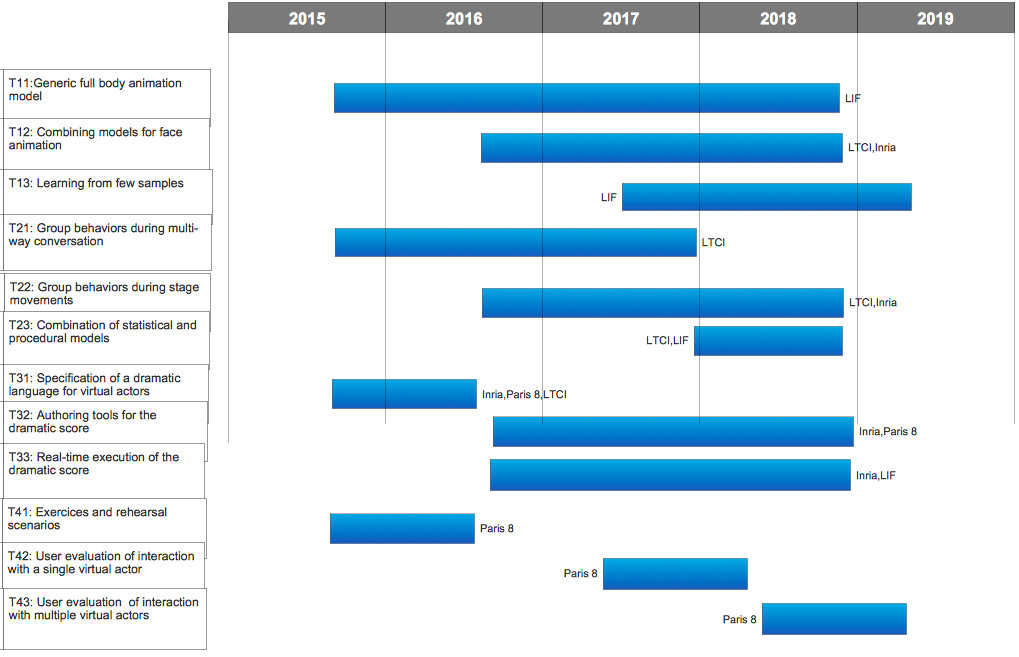
\includegraphics[width=\linewidth]{ganttdada.png}
\caption{GANTT diagram of tasks and ressources for DADA.}
\label{default}
\end{center}
\end{figure}


\subsubsection{Milestones}
 
The project will be organized in four main phases, separated by three milestones at $T_0+12$, $T_0+24$ and $T_0+36$:

\vspace{1cm}
\begin{center}
\begin{tabular}{|c|c|}
\hline
Phase 1 ($T_0 \rightarrow T_0+12$) & Specifications and scenarios. \\\hline
Milestone 1 ($T_0+12$) & Delivery of  specifications and scenarios.\\\hline
Phase 2 ($T_0+12 \rightarrow T_0+24$) & Research and development for first prototype.\\\hline
Milestone 2 ($T_0+24$) & Delivery of  first prototype.\\\hline
Phase 3 ($T_0+24 \rightarrow T_0+36$) & Research and development for second protoype.\\\hline
Milestone 3 ($T_0+36$) & Delivery of  second prototype.\\\hline
Phase 4 ($T_0+36  \rightarrow T_0+42$ & Final user evaluations.\\\hline
\end{tabular}
\end{center}


\subsubsection{Deliverables}
The project includes 12 deliverables which will be delivered at the three milestones. 

%\vspace{1cm}
\begin{center}
\begin{tabular}{|c|p{10cm}|c|c|}
\hline
Number & Title & Date & Leader\\\hline
L1.1  & Report on the state of the art for statistical models for animation synthesis &  $T_0+12$ & LIF\\\hline
L1.2  & First version of the models : Prototype (software) and its documentation (Report on the models developed) & $T_0+24 $  & LIF\\\hline
L1.3  & Second version of the models : Prototype (software) and its documentation (Report on the models developed)  & $T_0+36$ & LIF \\\hline
L2.1  & Report on the state of the art of proxemics models in computer animation&   $T_0+12$ & LITC \\\hline
L2.2  &  First version of the models : Prototype (software) and its documentation (Report on the models developed) & $T_0+24$ &LITC \\\hline
L2.3  &  Second version of the models : Prototype (software) and its documentation (Report on the models developed) &  $T_0+36$ & LITC \\\hline
L3.1  & Specification of the dramatic score language &  $T_0+12$  & Inria \\\hline
L3.2  & First version of authoring tools and execution environment : Prototype (software) and its documentation &  $T_0+24$  & Inria \\\hline
L3.3  & Second version of authoring tools and execution environment : Prototype (software) and its documentation &  $T_0+36$   & Inria \\\hline
L4.1  & Selection of example scenes and examples: collection of  one actor directing exercices   & $T0+12$ & Paris 8\\\hline
L4.2  & Preliminary revaluation report: Animated scenes with one actor, on the exercises defined in task 4.1. & $T0+30$ & Paris 8 \\\hline
L4.3  & Final evaluation report: Animated scenes with three virtual actors, showing exercises and selected examples from "L'augmentation" by Perec. & $T0+42$ & Paris 8 \\\hline
\end{tabular}
\end{center}



 
\endinput